
\section{Implementation}
We introduce the architecture of event-based workflow system and then discussed the details for every component. Figure 3 shows the architecture of event-driven workflow and it's work procedure.

\begin{figure} 
\centering
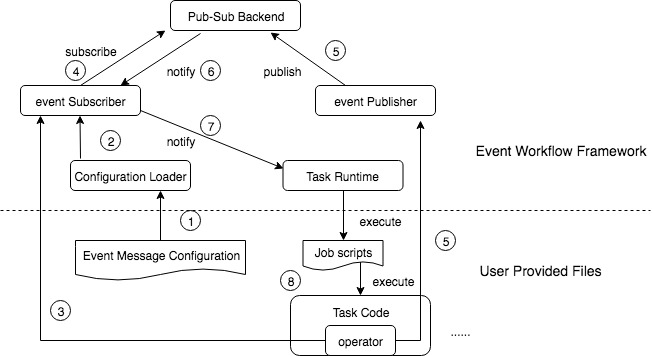
\includegraphics[width=1\linewidth]{./figure/edflowarchitecture.jpg}
\caption{Event driven workflow framework archetecture}
 \label{fg:state}
\end{figure} 


The user view and the workflow frame view are shown in Figure 3,  User needs to provide the initial configuration files which include the path of the job script and the event that every task interested, those events will be subscribed into the event store. The operator is the in-situ part integrated into the simulation code which is used to send subscribe and publish request during the simulation run. When specific events are published, the subscribing end will be notified and the job scripts will be started by task runtime. Several typical and in-situ using scenarios can be supported because this event pub-sub backend support pub-sub in 1:1, 1:n and n:1 manner and a user-defined event also provide flexibility to express the task dependency in fine-grained ways. 

(1) Traditional predefined static dependency tasks can be supported by running operator before task start running (subscribe event) after the task finish (publish event), the task will start running only when the specific event happens.

(2) The granularity of data dependency can be defined by the user in a flexible way to avoid post-processing and decrease all the workflow running time. For example, when every thread generates specific domain data, the visualization task can be notified and triggered immediately when all the subscribed events are satisfied.

More detailed using scenarios will be discussed in experiments and evaluation. We will introduce the key component for the following parts. 

\subsection{Optimised Pub-Sub Backend}

In this part, we introduce the design and implementation of optimized pub-sub mechanism and discuss how it supports both traditional and in-situ task dependency pattern in a workflow. Besides, we also leverage the canonical pub-sub mechanism and make it support the aggregation(fan-in) and broadcaster(fan-out) pattern at the same time, namely one event subscriber could subscribe multiple sub-event messages and specify the triggering conditions, when all the events are published specific times, the subscribed events will be triggered subsequently. The simplified underlying data structure is shown in Figure 6, eventually, we need to maintain several core maps to keep the mapping relation from one client id to several subscribed events and from one event to several client ID that interested to it. besides, we also need to use another map to record the published times for every event and use this info to check if the specific client should be notified. the subscribe and publish method is described as follows:

(1) event subscribe: For every subscribe request, there is a new id will be unique id will be generated and stored at back end, the event that this client interested will also be recorded and associated map will be initialised, there is a house-keeping logic in every subscribe method keeps checking the satisfactory flag, request will block here if the flag is not satisfied, otherwise the notify status will be returned back to client.

(2) event publish: When there is publish request, the backend will parse the event message in a request and retrieve the event from the map of an event to subscribe client id. For example, if we assume the publishing event is EVENTA. For every client id, we could get the event set it subscribed(every client is associated with an event message set), we could find EVENTA from this set and increase one for the number it is pushed, then we could check the required triggering number in published event, if the number equals to the required number, we could set the satisfied flag as true.

\subsection{Event Configuration and Data Operator}


\subsection{Task Runtime}
Task Runtime is designed to support multiple drivers to execute a task. The input of the task runtime is the driver name and the path of the running scripts. If the driver is the container solution such as Singularity or Docker, the execution path could be the name of the image.

